\section{Numerical  study}

We propose a simple simulation to illustrate the interest of using
multi-attribute networks and the efficiency of our proposal.  The
simulations are set up as follows:
\begin{enumerate}
\item  Draw  a random  undirected  network  with  $p$ nodes  from  the
  Erdös-Renyi model;
\item  Expand the  associated adjacency  matrix to  multivariate space
  with
  $$\mathbf{A} = \mathbf{A}  \otimes \mathbb{S} + \mathbf{I}_{p\times K}$$
  where $\otimes$ is the Kronecker product. The $K\times K$ matrix
  $\mathbb{S}$ is used to consider different scenarios of agreement
  across the attributes of two genes. We consider three cases
  \begin{enumerate}
  \item $\mathbb{S} = \mathbf{1}_{K,K}$ a matrix full of one (\emph{full} agreement)
  \item $\mathbb{S} = \mathbf{I}_{K,K}$ the $K\times K$ identity (\emph{independence} between  attributes)
  \item $\mathbb{S} = \mathbf{I}_{K,K} - \mathbf{1}_{K,K}$, (\emph{independence} across attributes)
  \end{enumerate}
\item Compute $\bTheta$ a positive definite approximation of
  $\mathbf{A}$ by replacing null and negative eigenvalues by a small constant;
\item Control the difficulty of  the problem with $\gamma>0$ such that
  $\bTheta= \bTheta+ \gamma I$;
\item  Draw  an i.i.d.   sample  $\bX$  of $X  \sim  \mathcal{N} \left( 0,\invcov^{-1} \right) .$
\end{enumerate}
We choose small networks with $p=20$, with $20$ edges on average and
vary $n$ from $p/2$ to $2p$. We consider cases where the number of
attributes is $K=2,3,4$.  We either apply neighborhood selection
procedure on each dimension separately and compute a mean AUC, or
neighborhood selection procedure on merge data then compute AUC, or
the multi-attribute counterpart with group-wise penalty
\eqref{eq:penalty_grp_variate} on the multivariate data.  We compute
the AUC for each method and replicate the experiment 100 times. On
Figure \ref{fig:simu_multi}, it is clear that aggregation improves
upon single-attribute methods.
% \begin{figure}[htbp!]
%   \centering
%   \begin{tabular}{cc}
%     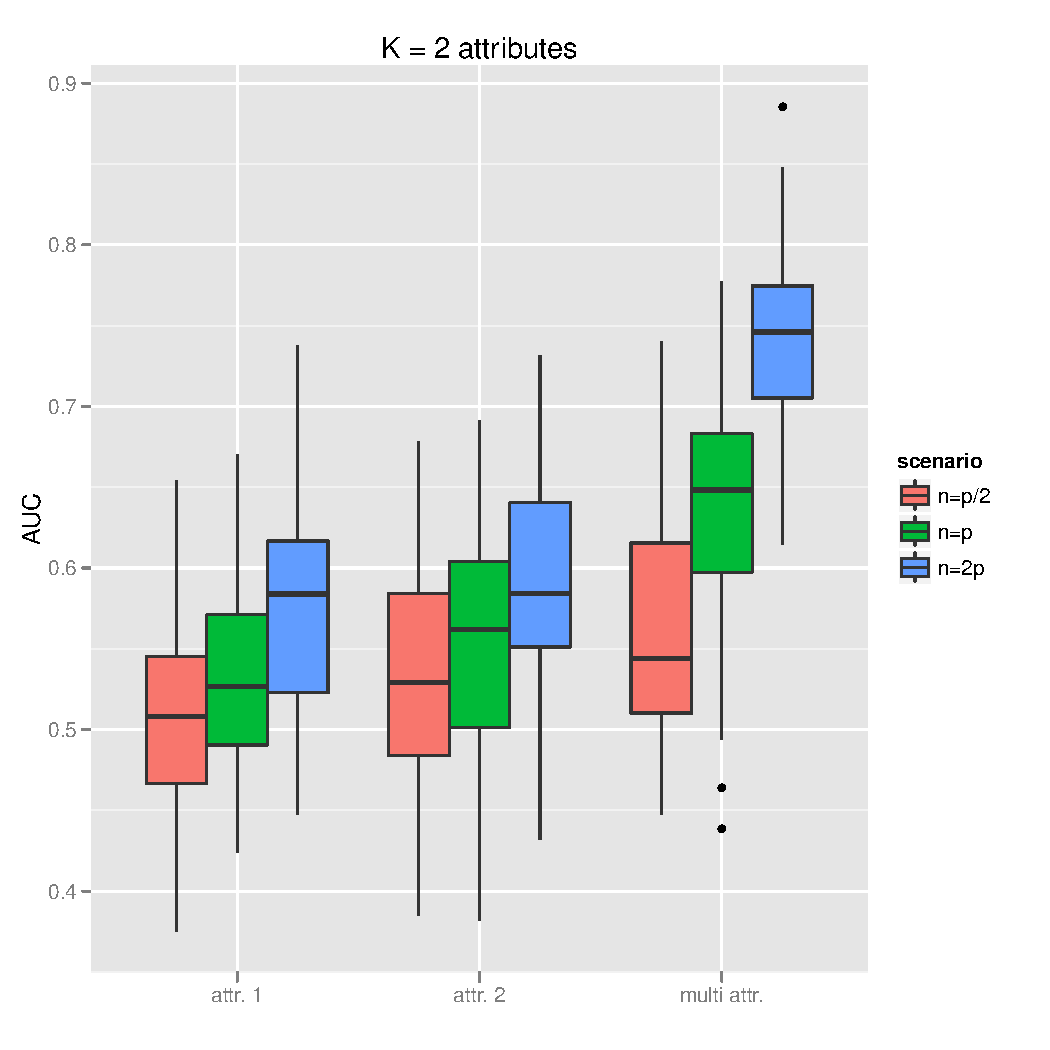
\includegraphics[width=.495\textwidth]{figures/res_simu_K=2} &
%     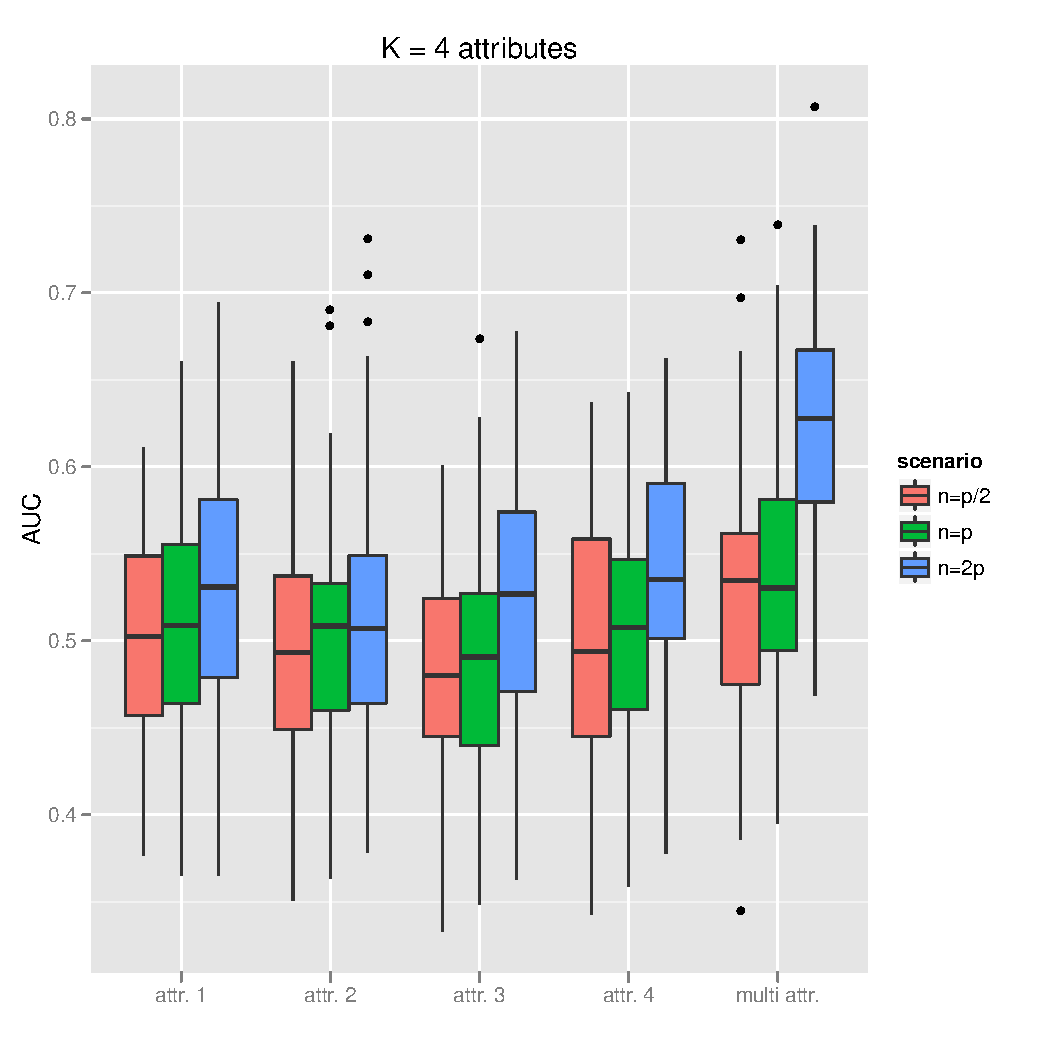
\includegraphics[width=.495\textwidth]{figures/res_simu_K=4} \\[1ex]
%     $K = 2$ & $K = 4$\\ 
%   \end{tabular}

%   \caption{Simple  simulation study  for  the multi-attribute  network
%     inference problem:  the multivariate  procedure improves  over the
%     univariate procedures in every  situation when networks are close
%     for each attribute.}
%   \label{fig:simu_multi}
% \end{figure}

\begin{figure}[htbp!]
  \centering
  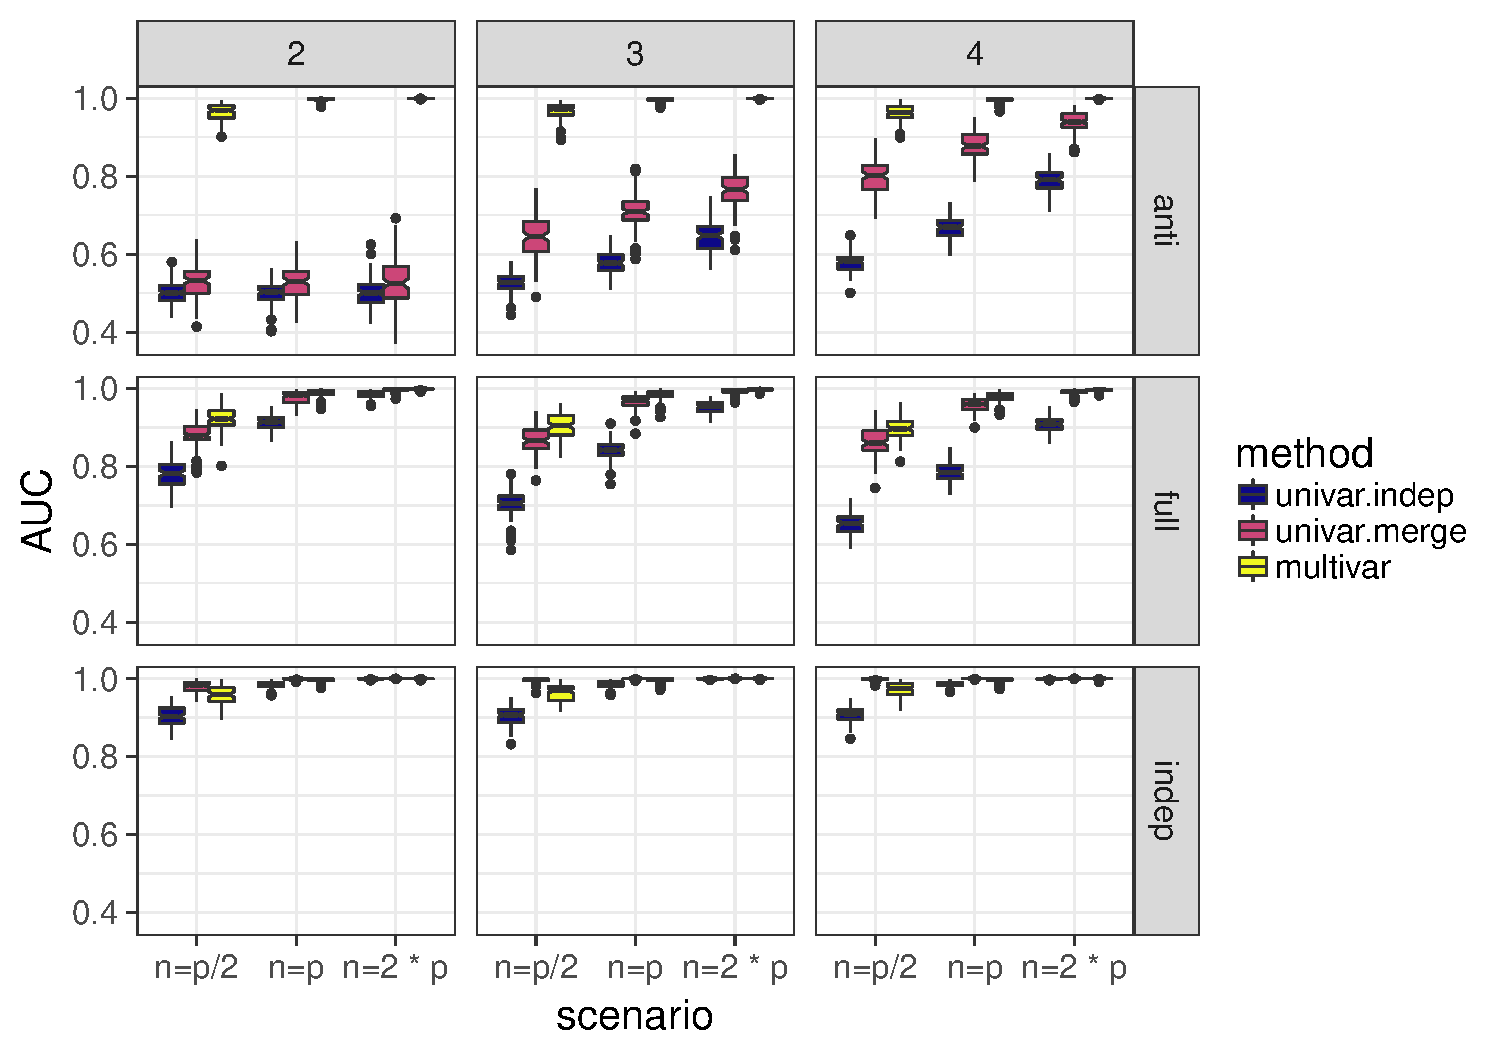
\includegraphics[width=\textwidth]{figures/res_simu_new}

  \caption{New simu... discuss this}
  \label{fig:simu_multi}
\end{figure}
